
\begin{frame}{Results}{Scenario 1 - Angle Range}

  \begin{block}{Goal}
	Describe the movement of the antennas when the UA is flying far away from the GS. 
  \end{block}

  \begin{figure}[H]
    \centerline{
    \subfigure[UAS Map]{
    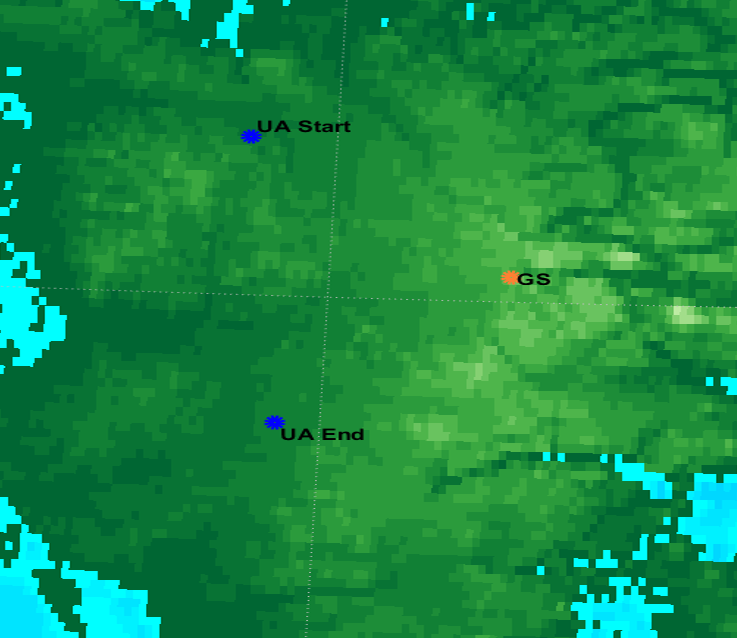
\includegraphics[scale=0.25]{figures/s1_zoom1.png}}
    \hfill
    \subfigure[Distance between UA and GS]{
    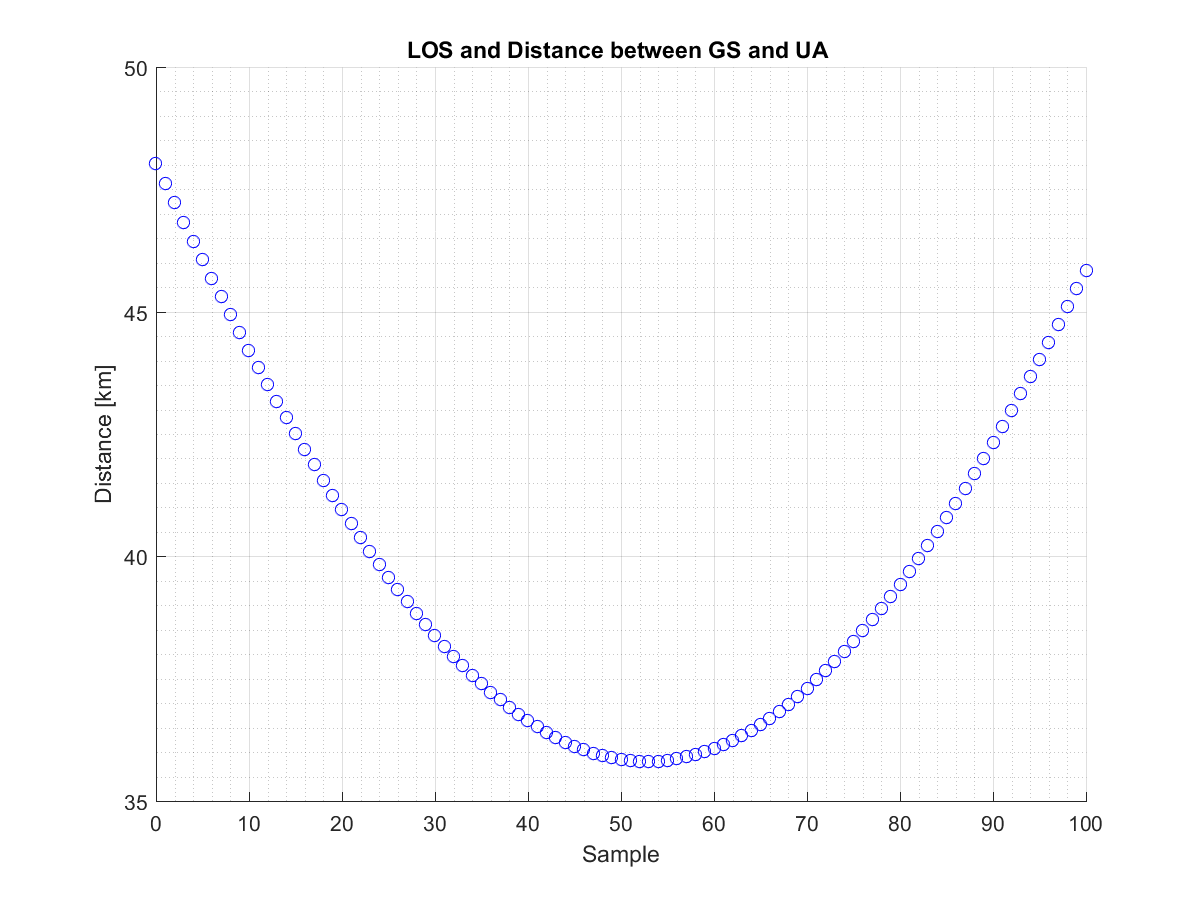
\includegraphics[scale=0.31]{figures/s1_los.png}}}
  \end{figure}

\end{frame}



\begin{frame}{Results}{Scenario 1 - Angle Range}

  \begin{block}{GS Tracking Angles}  
  
  \begin{figure}[H]
    \centerline{
    \subfigure[UAS Map]{
    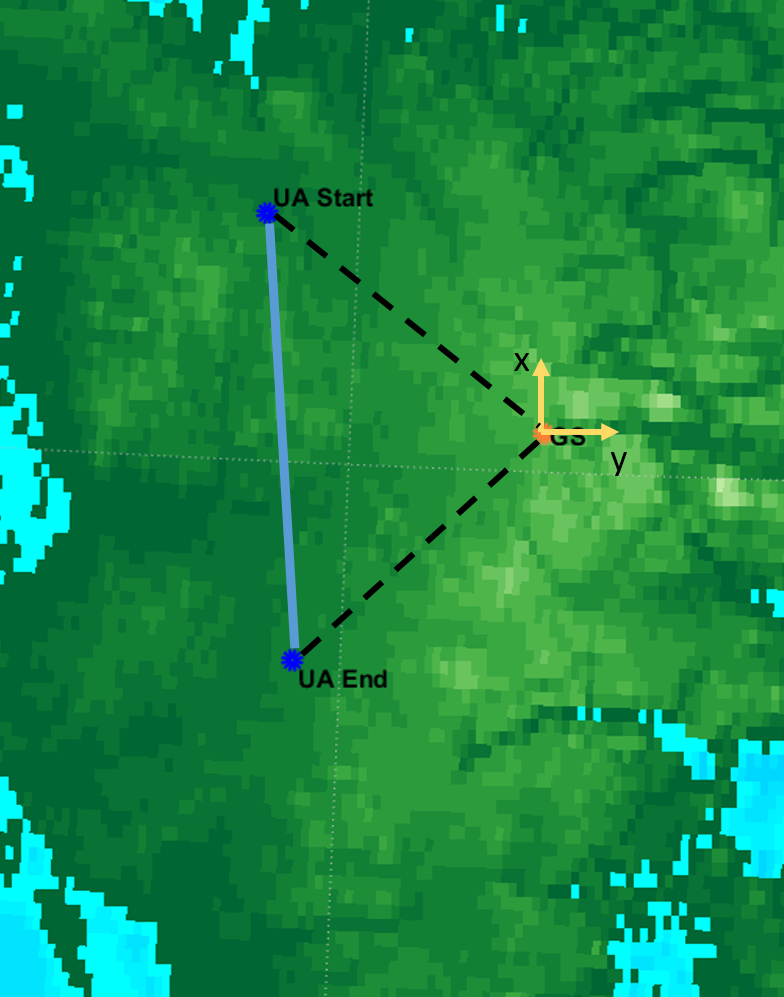
\includegraphics[scale=0.25]{figures/s1_zoom2.png}}
    \hfill
    \subfigure[Azimuth and elevation angles of the antenna on the GS]{
    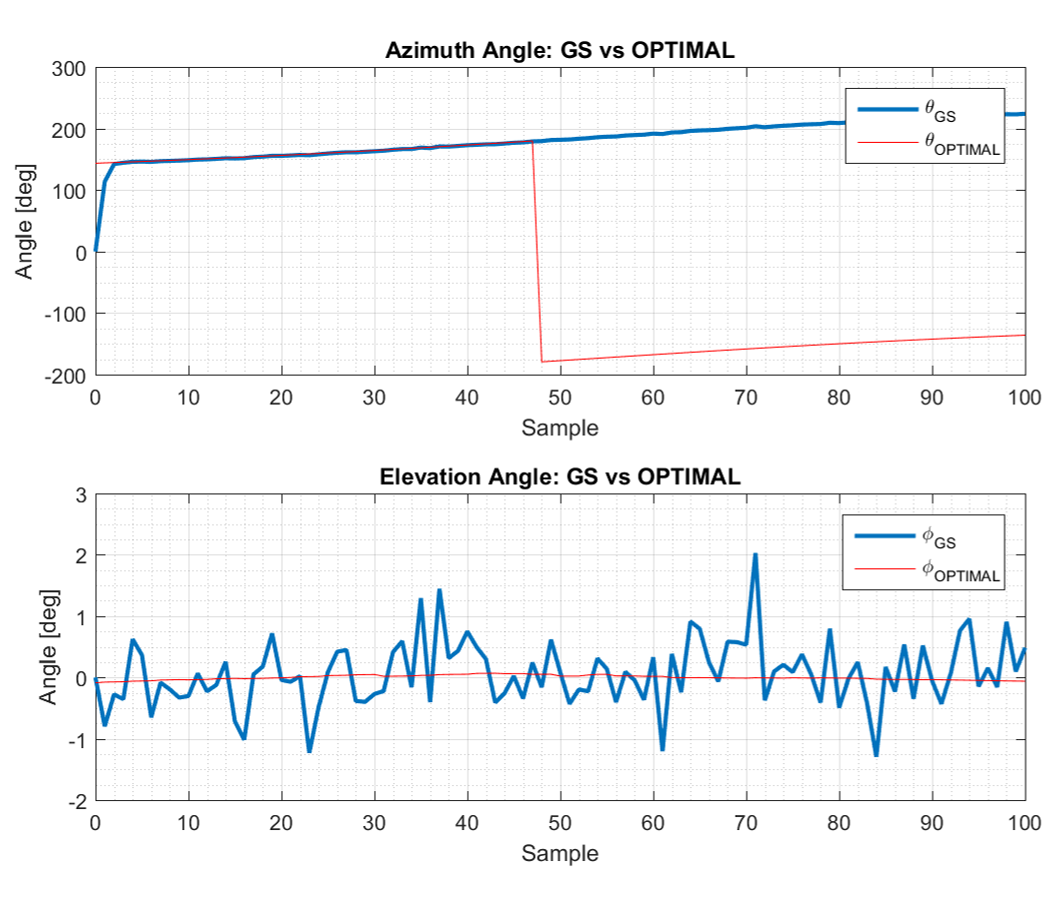
\includegraphics[scale=0.35]{figures/s1_pd_groundstation.png}}}
  \end{figure}
  
  \end{block}

\end{frame}



\begin{frame}{Results}{Scenario 1 - Angle Range}

  \begin{block}{GS Tracking Angles - Comparing PID Controllers}  
  
  \begin{figure}[H]
    \centerline{
    \subfigure[P Controller]{
    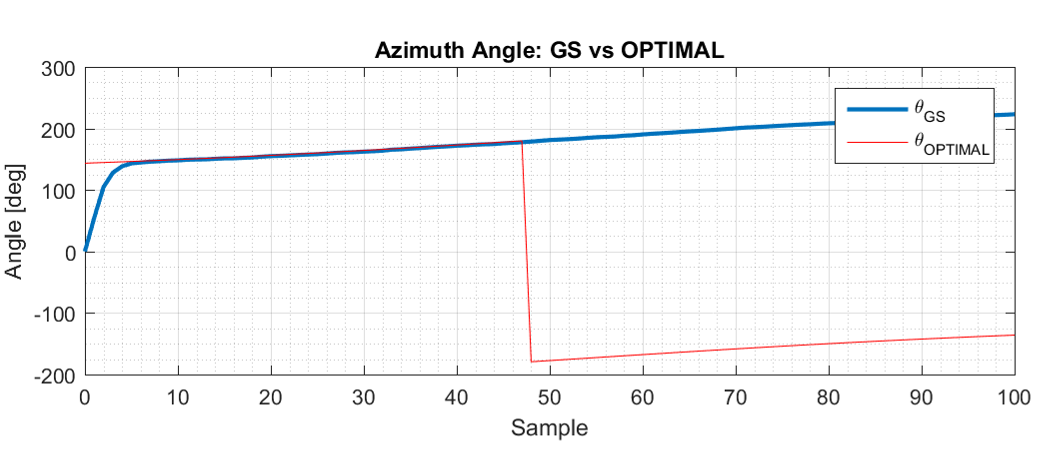
\includegraphics[scale=0.29]{figures/s1_p_gs.png}}
    \subfigure[PD Controller]{
    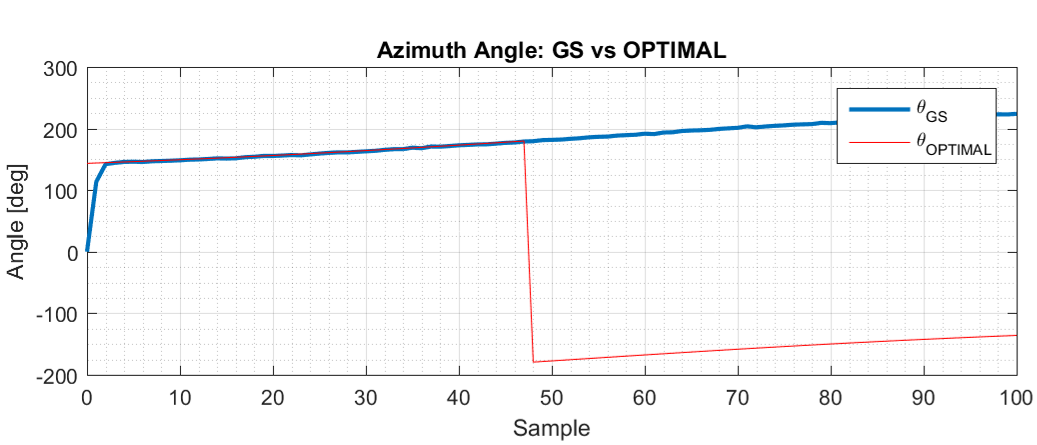
\includegraphics[scale=0.29]{figures/s1_pd_gs.png}}}
    \centerline{
    \subfigure[PI Controller]{
    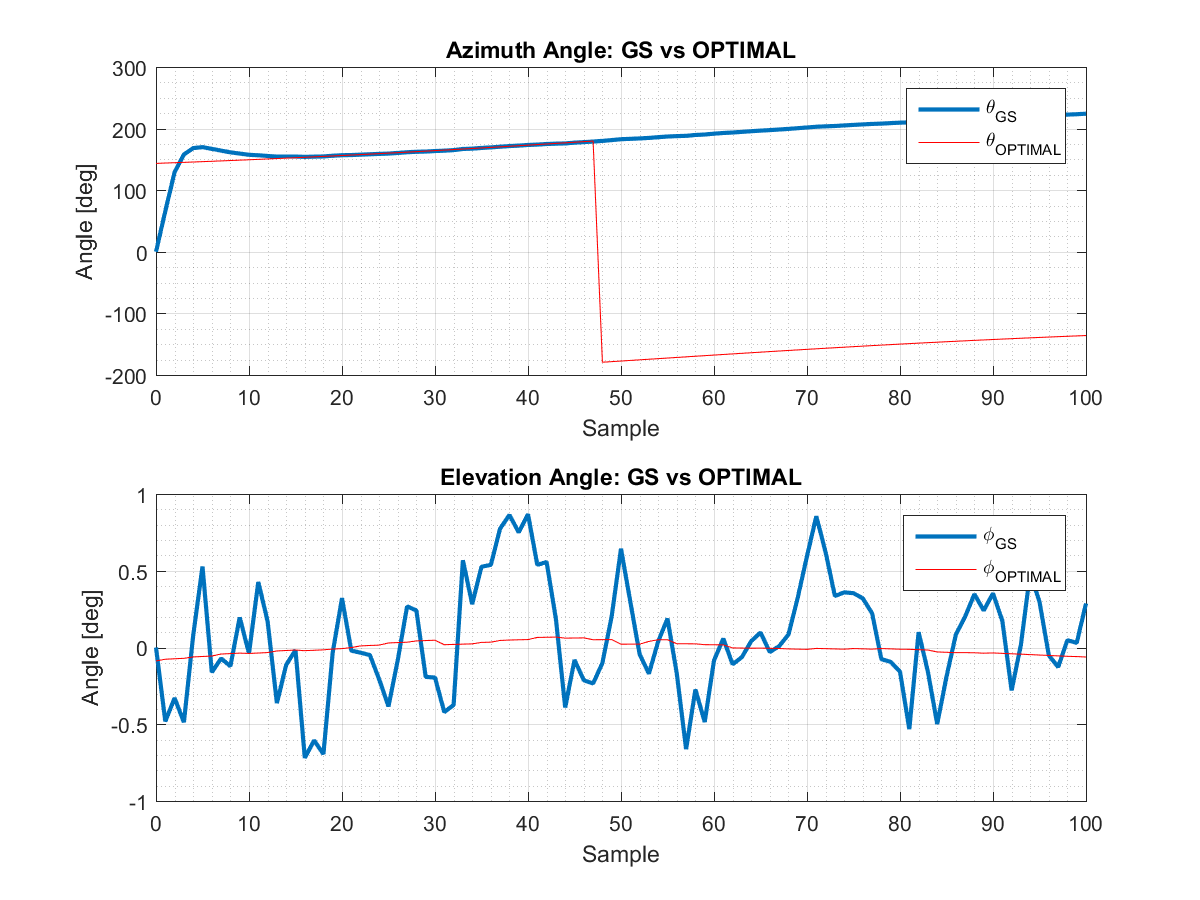
\includegraphics[scale=0.29]{figures/s1_pi_gs.png}}
    \subfigure[PID Controller]{
    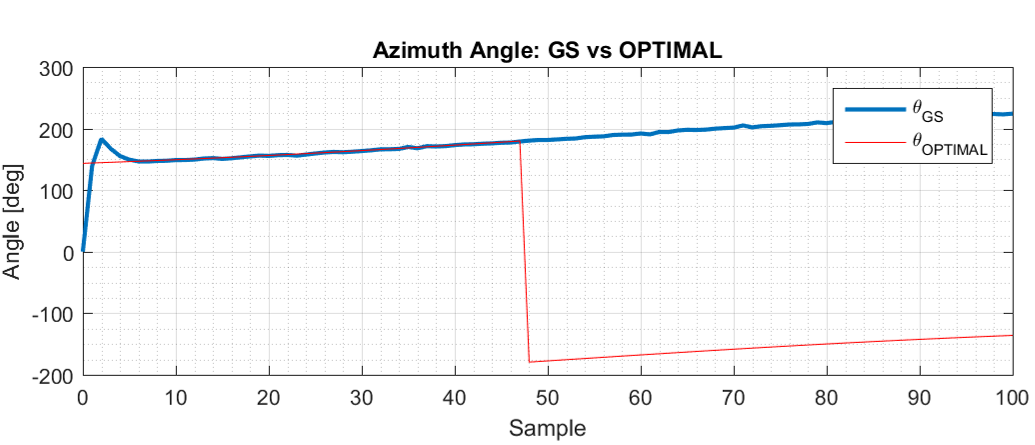
\includegraphics[scale=0.29]{figures/s1_pid_gs.png}}}
  \end{figure}
  
  \end{block}

\end{frame}



\begin{frame}{Results}{Scenario 1 - Angle Range}

  \begin{block}{UA Tracking Angles}  
  
  \begin{figure}[H]
    \centerline{
    \subfigure[UAS Map]{
    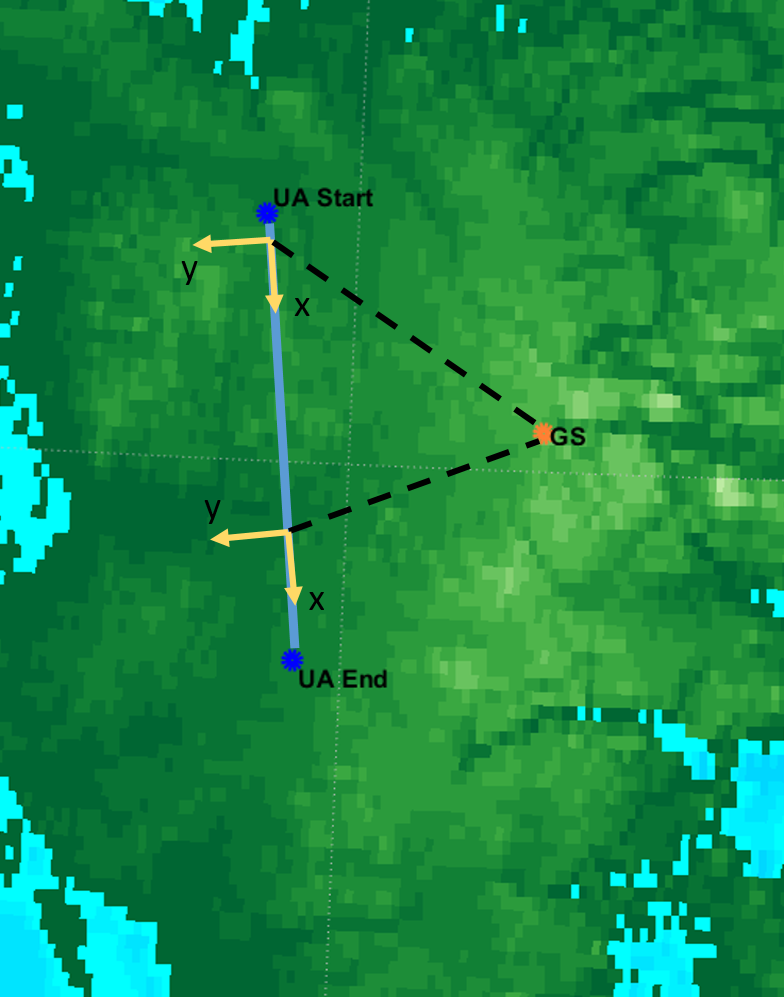
\includegraphics[scale=0.25]{figures/s1_zoom3.png}}
    \hfill
    \subfigure[Azimuth and elevation angles of the antenna on the UA]{
    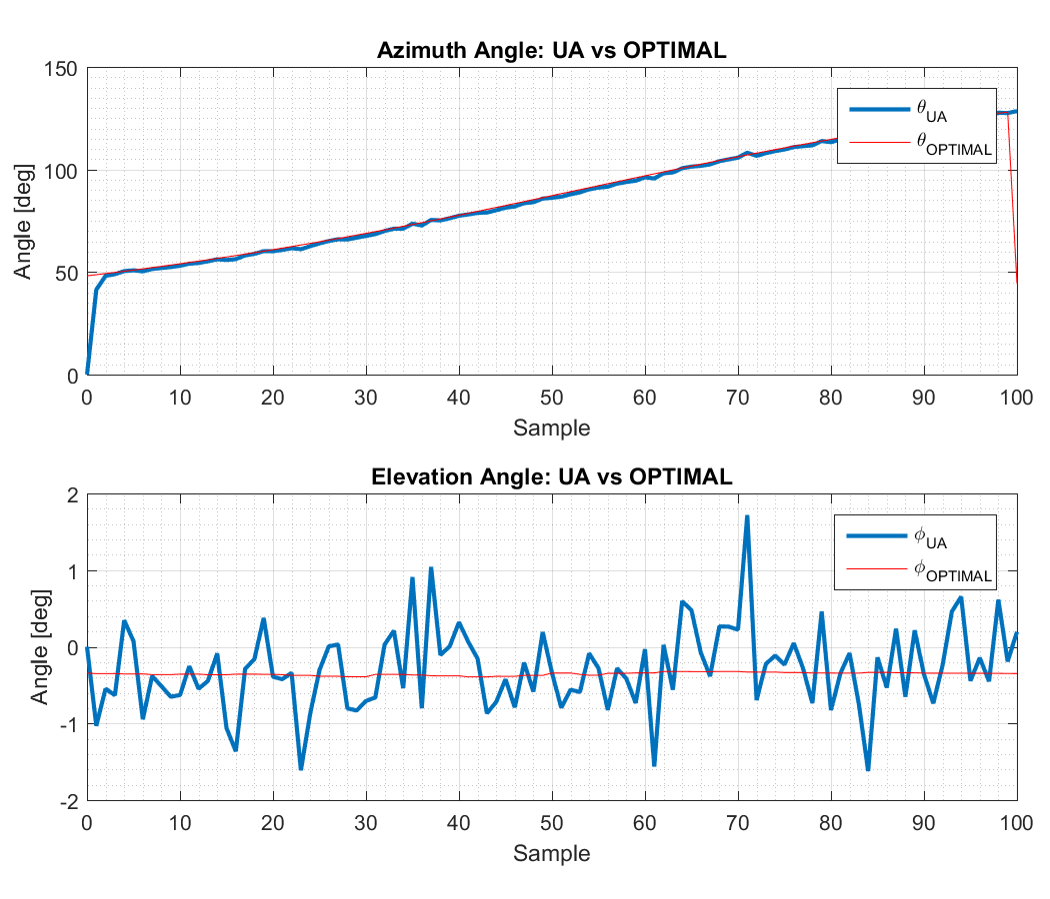
\includegraphics[scale=0.35]{figures/s1_pd_unmannedaircraft.png}}}
  \end{figure}
  
  \end{block}

\end{frame}



\begin{frame}{Results}{Scenario 1 - Angle Range}

  \begin{block}{UA Tracking Angles - Comparing PID Controllers}  
  
  \begin{figure}[H]
    \centerline{
    \subfigure[P Controller]{
    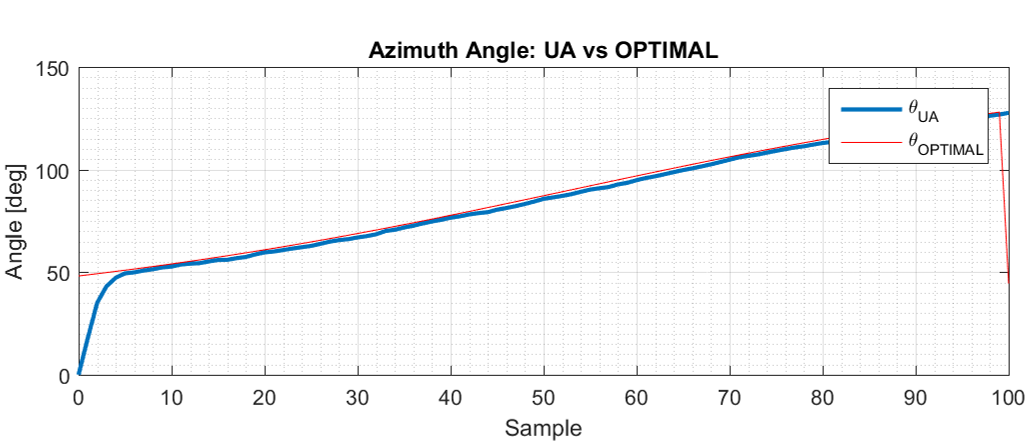
\includegraphics[scale=0.29]{figures/s1_p_ua.png}}
    \subfigure[PD Controller]{
    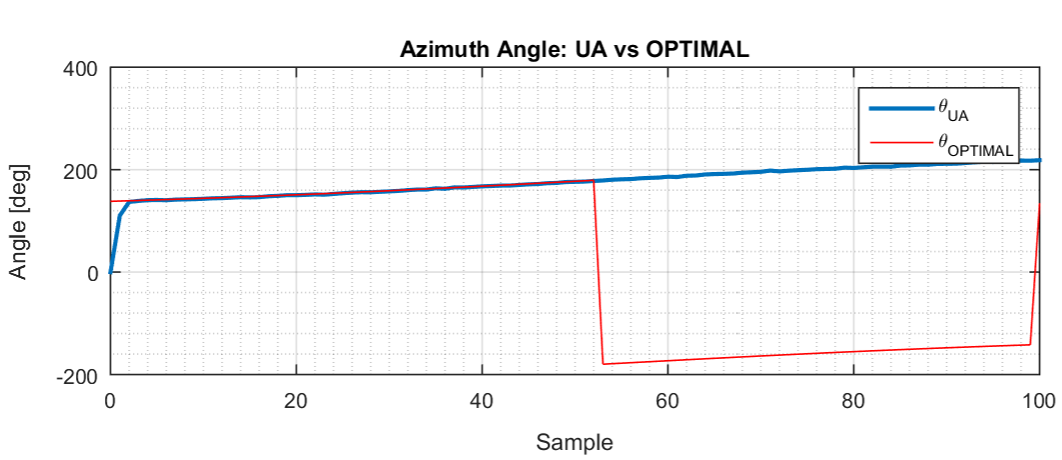
\includegraphics[scale=0.29]{figures/s1_pd_ua.png}}}
    \centerline{
    \subfigure[PI Controller]{
    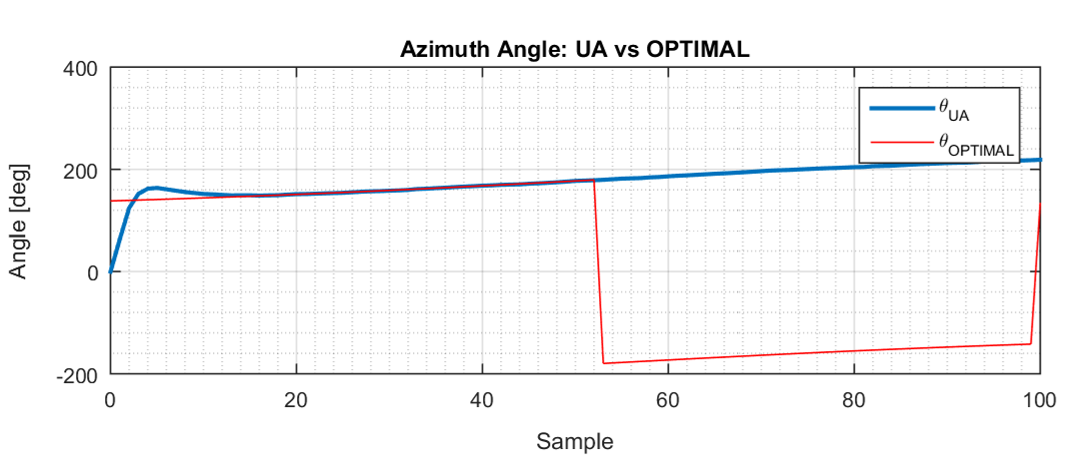
\includegraphics[scale=0.29]{figures/s1_pi_ua.png}}
    \subfigure[PID Controller]{
    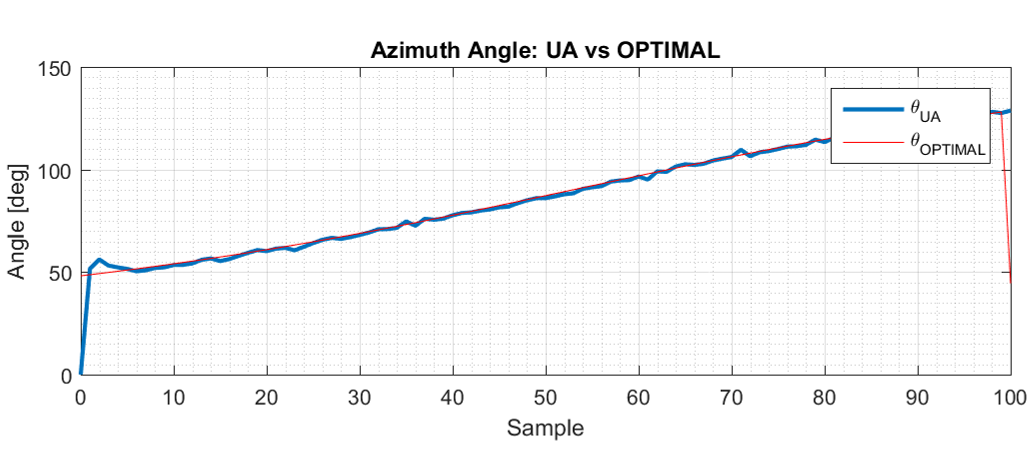
\includegraphics[scale=0.29]{figures/s1_pid_ua.png}}}
  \end{figure}
  
  \end{block}

\end{frame}



\begin{frame}{Results}{Scenario 1 - Angle Range}

  \begin{block}{Signal Power}  
  
  \begin{figure}[H]
    \centerline{
    \subfigure[UAS Map]{
    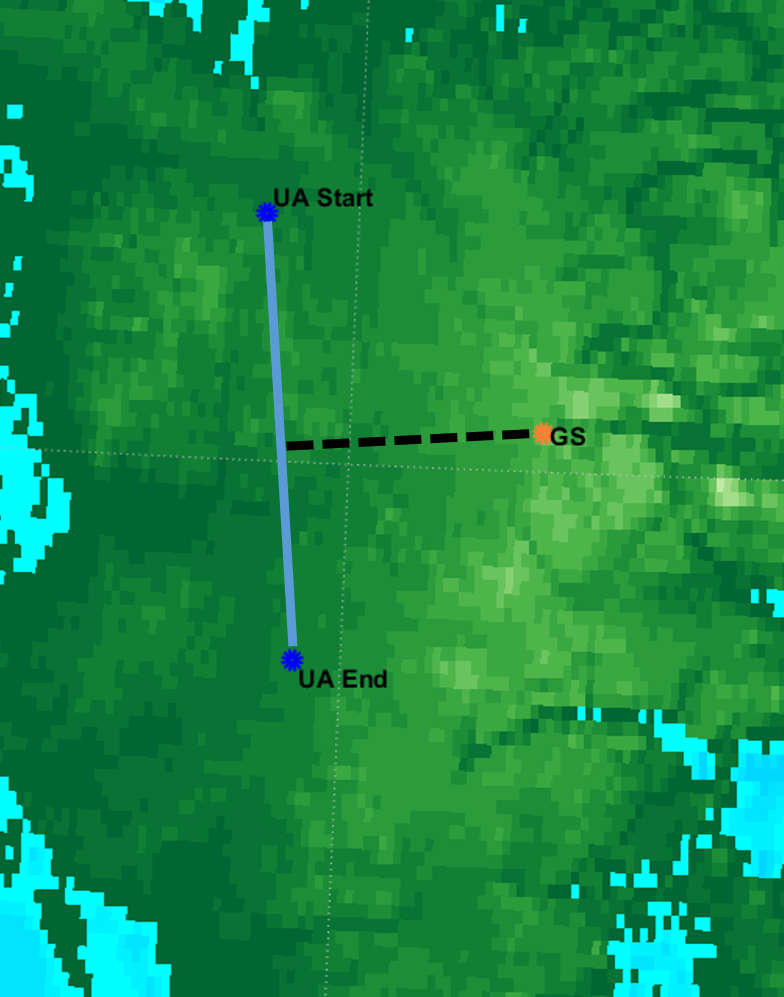
\includegraphics[scale=0.25]{figures/s1_zoom4.png}}
    \hfill
    \subfigure[Power at the receiver]{
    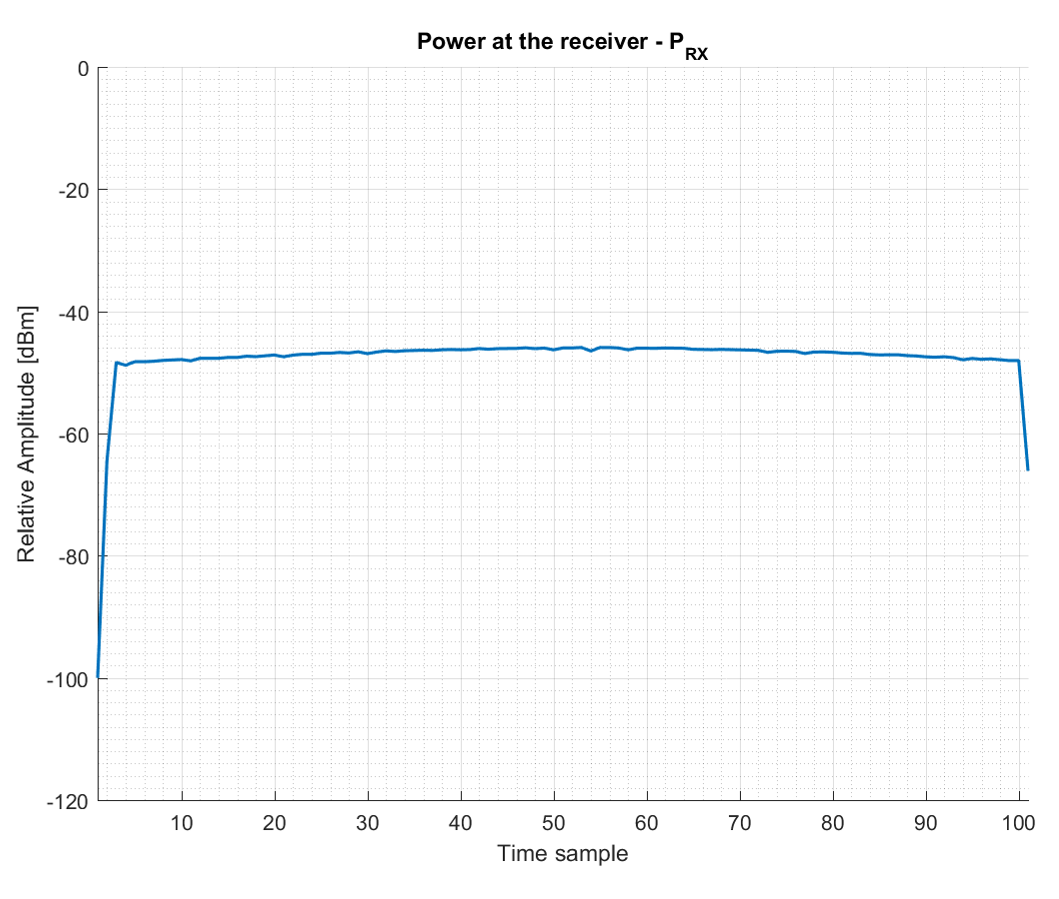
\includegraphics[scale=0.35]{figures/s1_pd_power.png}}}
  \end{figure}
  
  \end{block}

\end{frame}



\begin{frame}{Results}{Scenario 1 - Angle Range}

  \begin{block}{Signal Power - Comparing PID Controllers}  
  
  \begin{figure}[H]
    \centerline{
    \subfigure[P Controller]{
    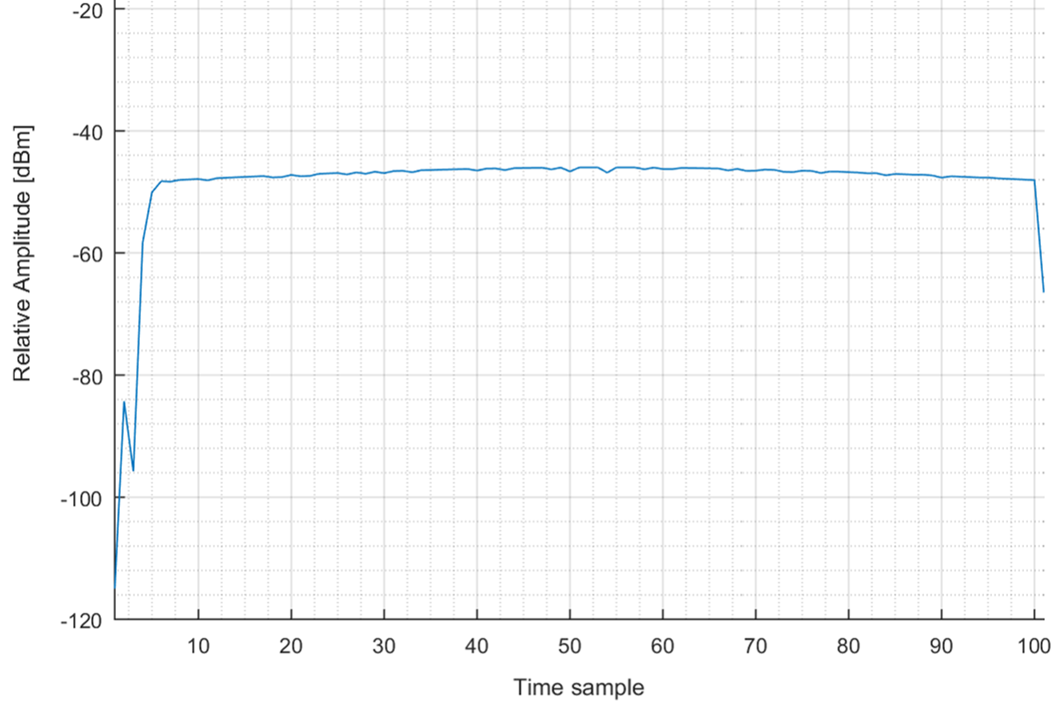
\includegraphics[scale=0.235]{figures/s1_p_power1.png}}
    \subfigure[PD Controller]{
    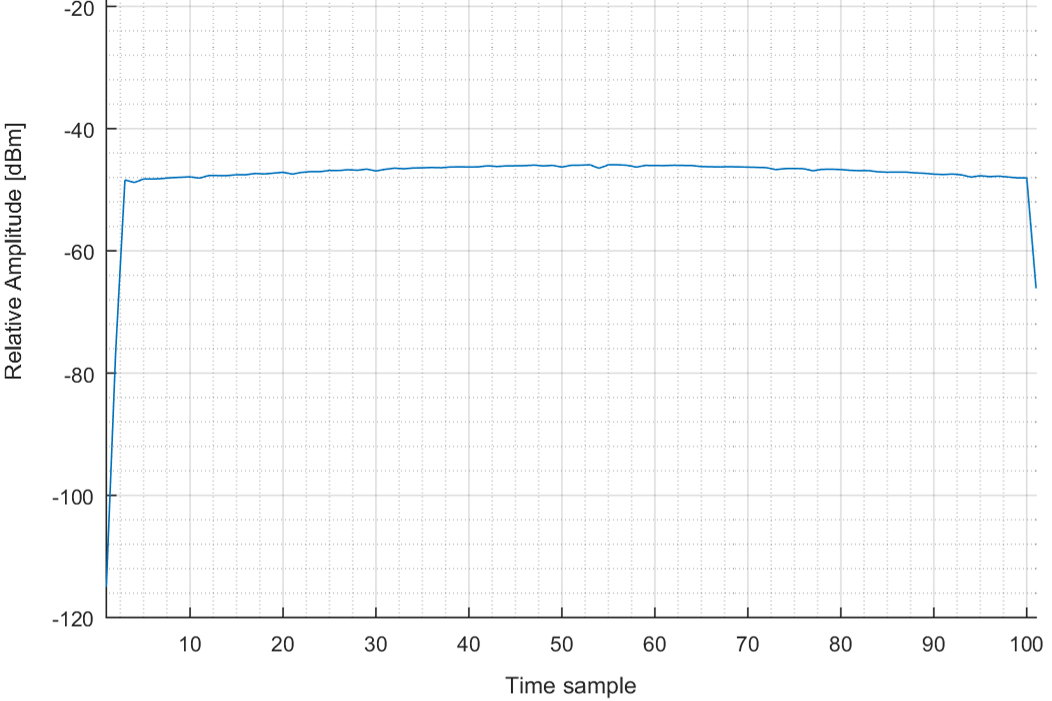
\includegraphics[scale=0.235]{figures/s1_pd_power1.png}}}
    \centerline{
    \subfigure[PI Controller]{
    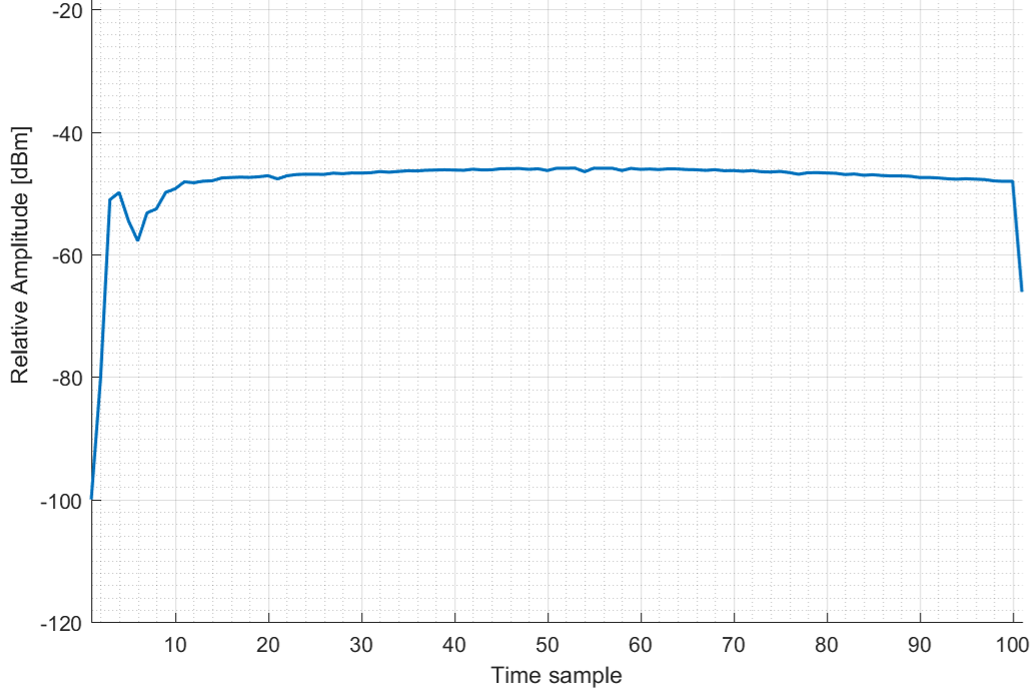
\includegraphics[scale=0.235]{figures/s1_pi_power1.png}}
    \subfigure[PID Controller]{
    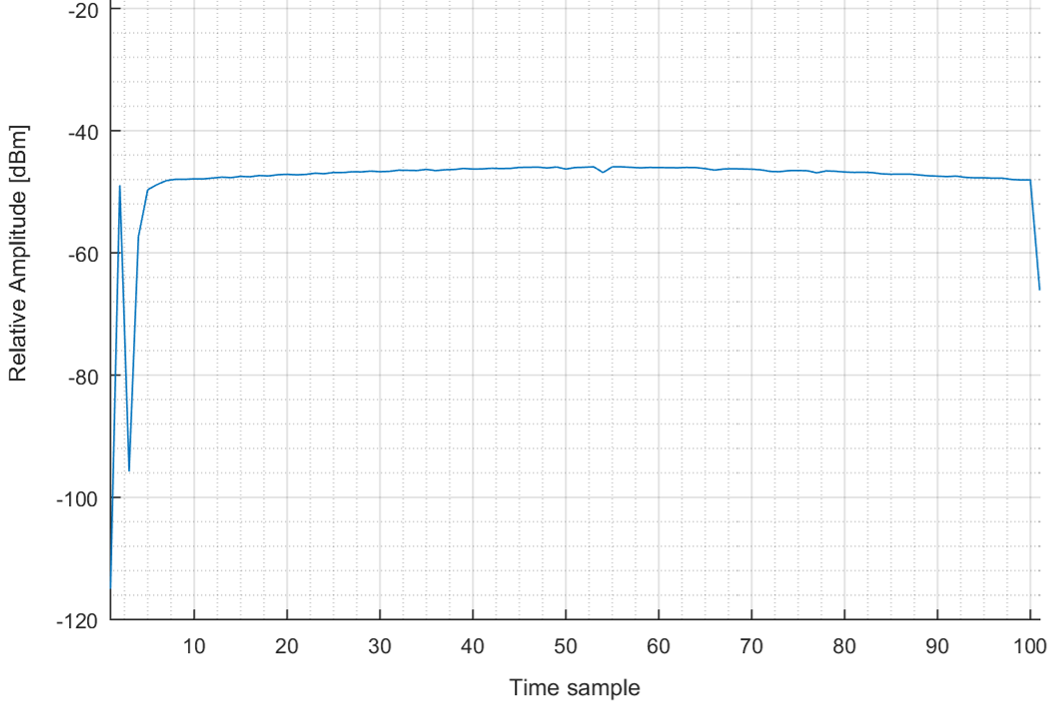
\includegraphics[scale=0.235]{figures/s1_pid_power1.png}}}
  \end{figure}
  
  \end{block}

\end{frame}